\documentclass[a4paper, 12pt]{exam}

\makeatletter
\expandafter\providecommand\expandafter*\csname ver@framed.sty\endcsname
{2003/07/21 v0.8a Simulated by exam}
\makeatother

\usepackage{xcolor}
\usepackage{minted}
\usepackage[utf8]{inputenc}
\usepackage{tikz}
\usepackage{caption}
\usepackage{gensymb}
\usepackage{lmodern}
\usepackage{multirow}
\usepackage{booktabs}
\usepackage{array}
\usepackage{adjustbox}
\usepackage{upquote}
\usepackage{amsmath}
\usepackage[hidelinks]{hyperref}
\usetikzlibrary{mindmap,shadows, shapes, arrows, automata, positioning, backgrounds}

\renewcommand{\refname}{\selectfont\normalsize References} 
\pagestyle{headandfoot}

\header{\textbf{Problem Sheet: Automata}}{}{Graph Theory}
\footer{}{Page \thepage\ of \numpages}{}
\marksnotpoints
\pointsinrightmargin

\begin{coverpages}
\end{coverpages}

\begin{document}

%\printanswers


\noindent These questions are largely taken from Sipser's book \cite{sipser96}.

\begin{questions}


\question
  Draw a DFA that accepts all strings over $\{a,b\}$ that have at least three $a$'s.
  
  \begin{solution}
    \begin{center}
      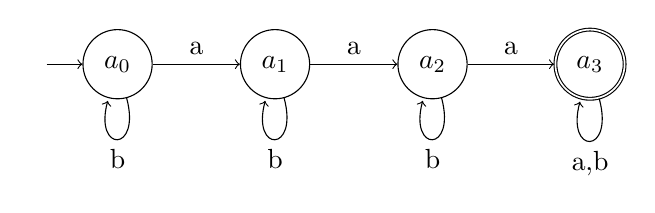
\begin{tikzpicture}[auto, on grid, node distance=2cm, initial text=]
        \node[state, initial]   (a_0)                {$a_0$}; 
        \node[state]            (a_1) [right of=a_0] {$a_1$};
        \node[state]            (a_2) [right of=a_1] {$a_2$}; 
        \node[state, accepting] (a_3) [right of=a_2] {$a_3$};
        \path[->] 
          (a_0) edge [loop below] node {b}   ()
                edge []           node {a}   (a_1)
          (a_1) edge [loop below] node {b}   ()
                edge []           node {a}   (a_2)
          (a_2) edge [loop below] node {b}   ()
                edge []           node {a}   (a_3)
          (a_3) edge [loop below] node {a,b} ();
      \end{tikzpicture}
    \end{center}
  \end{solution}

\question
  Draw a DFA that accepts all strings over $\{a,b\}$ that have at least two $b$'s.
  \begin{solution}
    \begin{center}
      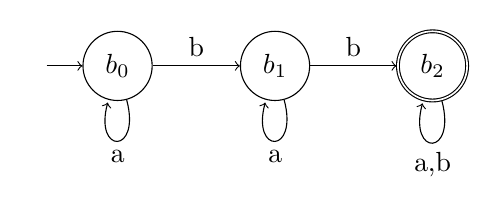
\begin{tikzpicture}[auto, on grid, node distance=2cm, initial text=]
        \node[state, initial]   (b_0)                {$b_0$}; 
        \node[state]            (b_1) [right of=b_0] {$b_1$};
        \node[state, accepting] (b_2) [right of=b_1] {$b_2$}; 
        \path[->] 
          (b_0) edge [loop below] node {a}   ()
                edge []           node {b}   (b_1)
          (b_1) edge [loop below] node {a}   ()
                edge []           node {b}   (b_2)
          (b_2) edge [loop below] node {a,b} ();
        \end{tikzpicture}
      \end{center}
  \end{solution}

\question
  Draw a DFA that accepts all strings over $\{a,b\}$ that have exactly two $a$'s.
  \begin{solution}
    \begin{center}
      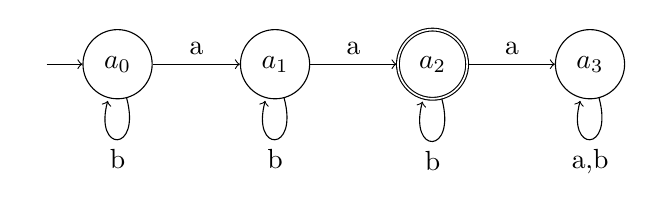
\begin{tikzpicture}[auto, on grid, node distance=2cm, initial text=]
        \node[state, initial]   (a_0)                {$a_0$}; 
        \node[state]            (a_1) [right of=a_0] {$a_1$};
        \node[state, accepting] (a_2) [right of=a_1] {$a_2$}; 
        \node[state]            (a_3) [right of=a_2] {$a_3$};
        \path[->] 
          (a_0) edge [loop below] node {b}   ()
                edge []           node {a}   (a_1)
          (a_1) edge [loop below] node {b}   ()
                edge []           node {a}   (a_2)
          (a_2) edge [loop below] node {b}   ()
                edge []           node {a}   (a_3)
          (a_3) edge [loop below] node {a,b} ();
      \end{tikzpicture}
    \end{center}
  \end{solution}

  \question
  Draw a DFA that accepts all strings over $\{a,b\}$ that have an odd number of $a$'s.
  \begin{solution}
    \begin{center}
      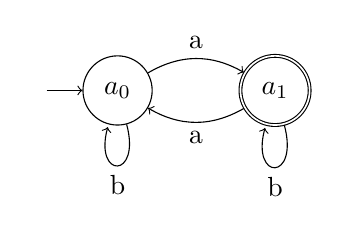
\begin{tikzpicture}[auto, on grid, node distance=2cm, initial text=]
        \node[state, initial]   (a_0)                {$a_0$}; 
        \node[state, accepting] (a_1) [right of=a_0] {$a_1$};
        \path[->]
          (a_0) edge [bend left]  node {a} (a_1)
                edge [loop below] node {b} (a_0)
          (a_1) edge [bend left]  node {a} (a_0)
                edge [loop below] node {b} (a_1);
      \end{tikzpicture}
    \end{center}
\end{solution}

\question
  Draw a DFA that accepts all strings over $\{a,b\}$ that have at least three $a$'s and at least two $b$'s.
\begin{solution}
  \begin{center}
    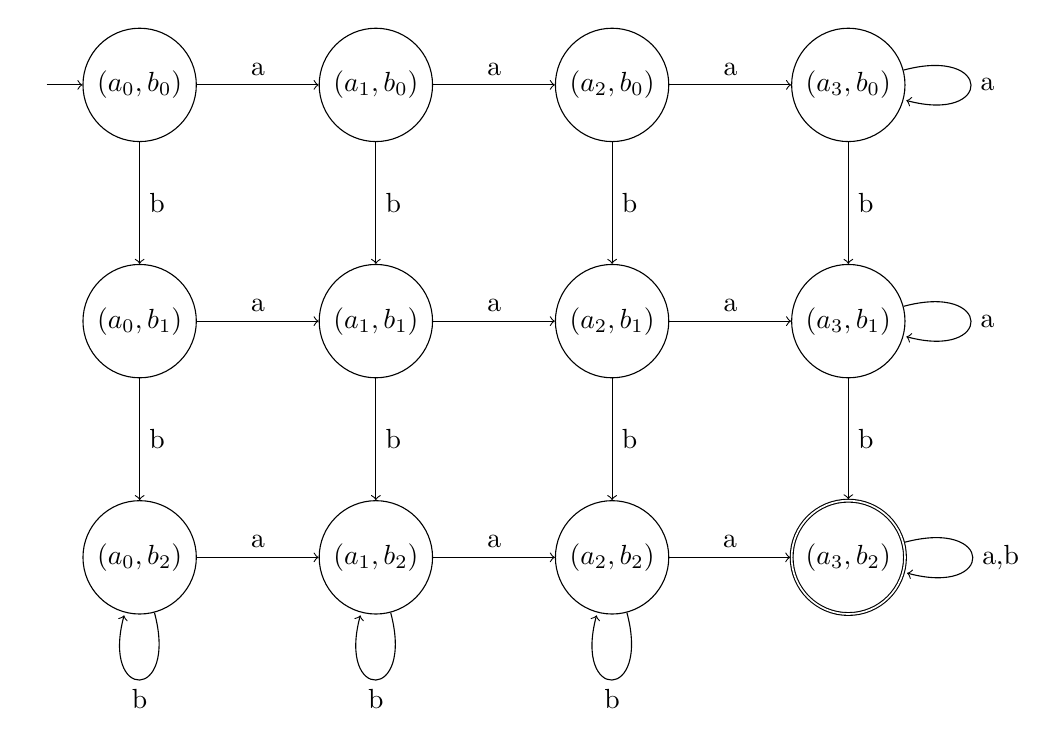
\begin{tikzpicture}[auto, on grid, node distance=3cm, initial text=]
      \node[state, initial]   (a0b0)                 {$(a_0,b_0)$};
      \node[state]            (a1b0) [right of=a0b0] {$(a_1,b_0)$};
      \node[state]            (a2b0) [right of=a1b0] {$(a_2,b_0)$};
      \node[state]            (a3b0) [right of=a2b0] {$(a_3,b_0)$};

      \node[state]            (a0b1) [below of=a0b0] {$(a_0,b_1)$};
      \node[state]            (a1b1) [right of=a0b1] {$(a_1,b_1)$};
      \node[state]            (a2b1) [right of=a1b1] {$(a_2,b_1)$};
      \node[state]            (a3b1) [right of=a2b1] {$(a_3,b_1)$};

      \node[state]            (a0b2) [below of=a0b1] {$(a_0,b_2)$};
      \node[state]            (a1b2) [right of=a0b2] {$(a_1,b_2)$};
      \node[state]            (a2b2) [right of=a1b2] {$(a_2,b_2)$};
      \node[state, accepting] (a3b2) [right of=a2b2] {$(a_3,b_2)$};
      \path[->] 
        (a0b0) edge []           node {a}   (a1b0)
              edge []           node {b}   (a0b1)
        (a0b1) edge []           node {a}   (a1b1)
              edge []           node {b}   (a0b2)
        (a0b2) edge []           node {a}   (a1b2)
              edge [loop below] node {b}   (a0b2)
        (a1b0) edge []           node {a}   (a2b0)
              edge []           node {b}   (a1b1)
        (a1b1) edge []           node {a}   (a2b1)
              edge []           node {b}   (a1b2)
        (a1b2) edge []           node {a}   (a2b2)
              edge [loop below] node {b}   (a1b2)
        (a2b0) edge []           node {a}   (a3b0)
              edge []           node {b}   (a2b1)
        (a2b1) edge []           node {a}   (a3b1)
              edge []           node {b}   (a2b2)
        (a2b2) edge []           node {a}   (a3b2)
              edge [loop below] node {b}   (a2b2)
        (a3b0) edge [loop right] node {a}   (a3b0)
              edge []           node {b}   (a3b1)
        (a3b1) edge [loop right] node {a}   (a3b1)
              edge []           node {b}   (a3b2)
        (a3b2) edge [loop right] node {a,b} (a3b2);
    \end{tikzpicture}
  \end{center}
\end{solution}

\question
  Define all of the above automata.

\question
  Draw an NFA that recognises, over the alphabet $\{0,1\}$, both strings that begin with a 1 and end with a 0 and strings that contain at least three 1's.
  \begin{solution}
    \begin{center}
  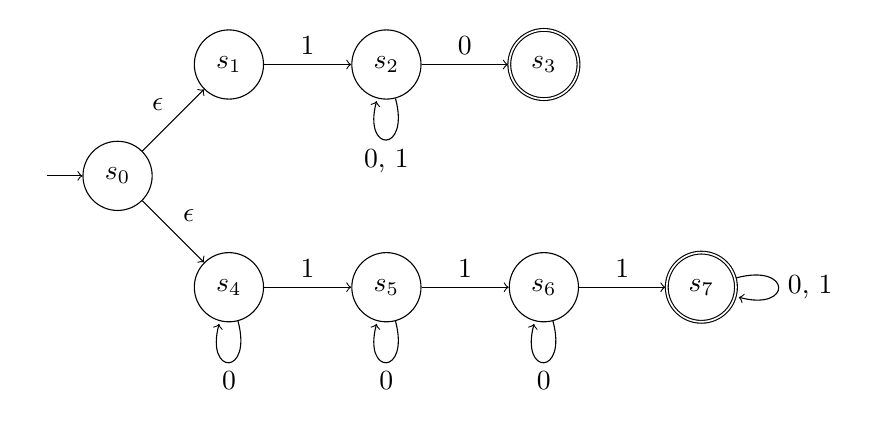
\begin{tikzpicture}[auto, on grid, node distance=2cm, initial text=]
      \node[state, initial]   (s_0)                      {$s_0$};
      \node[state]            (s_1) [above right of=s_0] {$s_1$};
      \node[state]            (s_2) [right of=s_1]       {$s_2$};
      \node[state, accepting] (s_3) [right of=s_2]       {$s_3$};
      \node[state]            (s_4) [below right of=s_0] {$s_4$};
      \node[state]            (s_5) [right of=s_4]       {$s_5$};
      \node[state]            (s_6) [right of=s_5]       {$s_6$};
      \node[state, accepting] (s_7) [right of=s_6]       {$s_7$};
      \path[->]
        (s_0) edge []           node {$\epsilon$} (s_1)
              edge []           node {$\epsilon$} (s_4)
        (s_1) edge []           node {1}          (s_2)
        (s_2) edge [loop below] node {0, 1}       (s_2)
              edge []           node {0}          (s_3)
        (s_4) edge [loop below] node {0}          (s_4)
              edge []           node {1}          (s_5)
        (s_5) edge [loop below] node {0}          (s_5)
              edge []           node {1}          (s_6)
        (s_6) edge [loop below] node {0}          (s_6)
              edge []           node {1}          (s_7)
        (s_7) edge [loop right] node {0, 1}       (s_7);
    \end{tikzpicture}
  \end{center}
\end{solution}


\question
  Draw an NFA that recognises, over the alphabet $\{0,1\}$, both strings that contain the substring 0101 and strings that don't contain the substring 110.
  \begin{solution}
    \begin{center}
      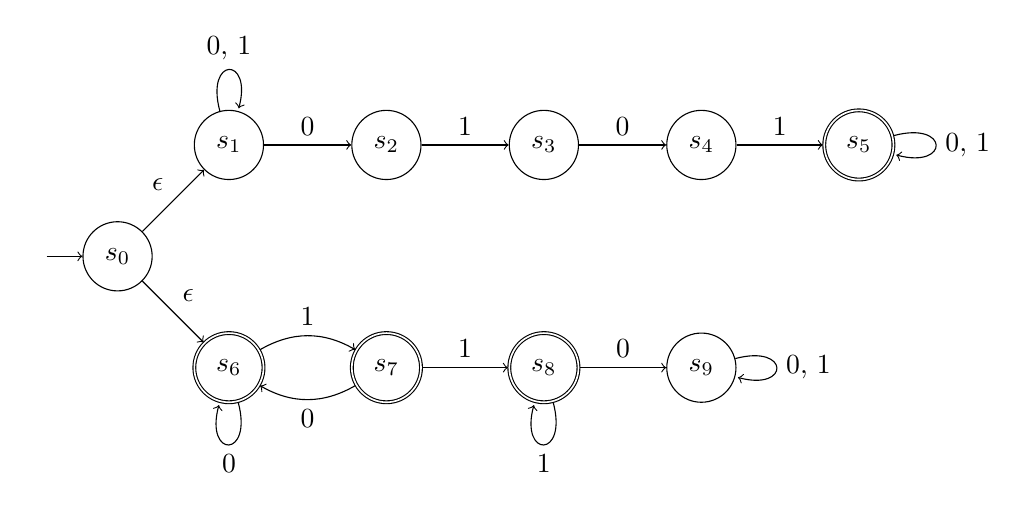
\begin{tikzpicture}[auto, on grid, node distance=2cm, initial text=]
        \node[state, initial]   (s_0)                      {$s_0$};
        \node[state]            (s_1) [above right of=s_0] {$s_1$};
        \node[state]            (s_2) [right of=s_1]       {$s_2$};
        \node[state]            (s_3) [right of=s_2]       {$s_3$};
        \node[state]            (s_4) [right of=s_3]       {$s_4$};
        \node[state, accepting] (s_5) [right of=s_4]       {$s_5$};
        \node[state, accepting] (s_6) [below right of=s_0] {$s_6$};
        \node[state, accepting] (s_7) [right of=s_6]       {$s_7$};
        \node[state, accepting] (s_8) [right of=s_7]       {$s_8$};
        \node[state]            (s_9) [right of=s_8]       {$s_9$};
        \path[->]
          (s_0) edge []           node {$\epsilon$} (s_1)
                edge []           node {$\epsilon$} (s_6)
          (s_1) edge [loop above] node {0, 1}       (s_1)
                edge []           node {0}          (s_2)
          (s_2) edge []           node {1}          (s_3)
          (s_3) edge []           node {0}          (s_4)
          (s_4) edge []           node {1}          (s_5)
          (s_5) edge [loop right] node {0, 1}       (s_5)
          (s_6) edge [loop below] node {0}          (s_6)
                edge [bend left]  node {1}          (s_7)
          (s_7) edge [bend left]  node {0}          (s_6)
                edge []           node {1}          (s_8)
          (s_8) edge []           node {0}          (s_9)
                edge [loop below] node {1}          (s_8)
          (s_9) edge [loop right] node {0, 1}       (s_9);
      \end{tikzpicture}
    \end{center}
  \end{solution}


\question
  Draw an NFA that recognises, over the alphabet $\{0,1\}$, the concatenations of strings of length at most five and strings where every odd position is a 1.
  \begin{solution}
    \begin{center}
    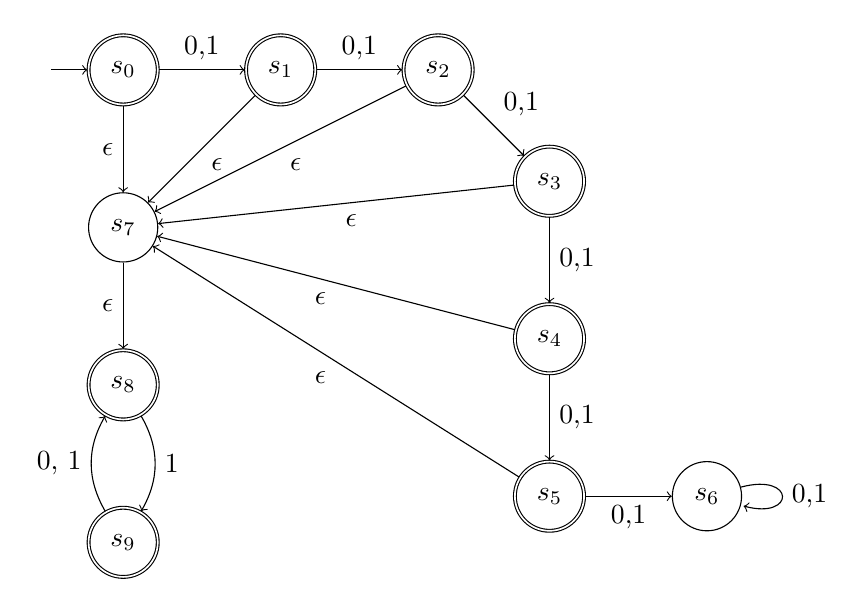
\begin{tikzpicture}[auto, on grid, node distance=2cm, initial text=]
      \node[state, initial, accepting]   (s_0)           {$s_0$};
      \node[state, accepting] (s_1) [right of=s_0]       {$s_1$};
      \node[state, accepting] (s_2) [right of=s_1]       {$s_2$};
      \node[state, accepting] (s_3) [below right of=s_2] {$s_3$};
      \node[state, accepting] (s_4) [below of=s_3]       {$s_4$};
      \node[state, accepting] (s_5) [below of=s_4]       {$s_5$};
      \node[state]            (s_6) [right of=s_5]       {$s_6$};
      \node[state]            (s_7) [below of=s_0]       {$s_7$};
      \node[state, accepting] (s_8) [below of=s_7]       {$s_8$};
      \node[state, accepting] (s_9) [below of=s_8]       {$s_9$};
      \path[->]
        (s_0) edge []           node {0,1}        (s_1)
              edge [swap]       node {$\epsilon$} (s_7)
        (s_1) edge []           node {0,1}        (s_2)
              edge []           node {$\epsilon$} (s_7)
        (s_2) edge []           node {0,1}        (s_3)
              edge []           node {$\epsilon$} (s_7)
        (s_3) edge []           node {0,1}        (s_4)
              edge []           node {$\epsilon$} (s_7)
        (s_4) edge []           node {0,1}        (s_5)
              edge []           node {$\epsilon$} (s_7)
        (s_5) edge [swap]       node {0,1}        (s_6)
              edge []           node {$\epsilon$} (s_7)
        (s_6) edge [loop right] node {0,1}        (s_6)
        (s_7) edge [swap]       node {$\epsilon$} (s_8)
        (s_8) edge [bend left]  node {1}          (s_9)
        (s_9) edge [bend left]  node {0, 1}       (s_8);
    \end{tikzpicture}
    \end{center}
  \end{solution}


  \question
  Draw an NFA that recognises, over the alphabet $\{0,1\}$, the Kleene star of the language containing strings with at least two 0's and at most one 1.
  \begin{solution}
    \begin{center}
    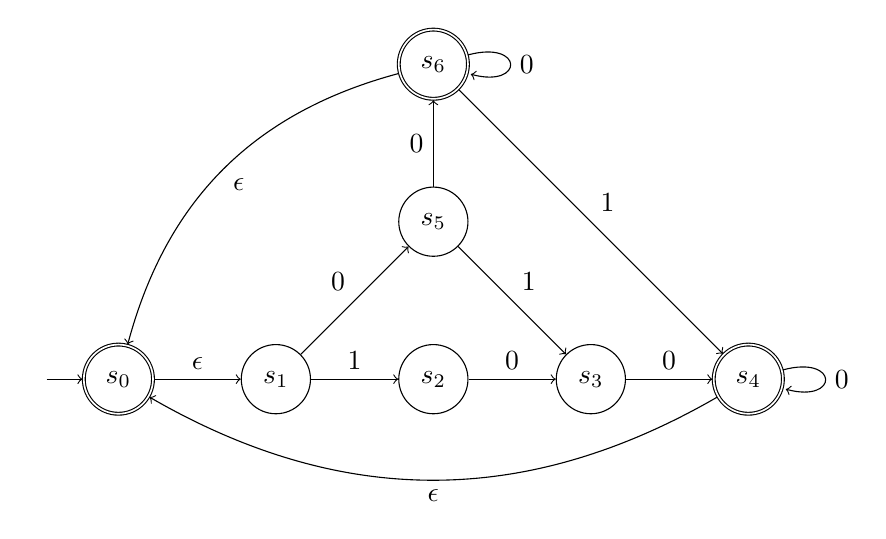
\begin{tikzpicture}[auto, on grid, node distance=2cm, initial text=]
      \node[state, initial, accepting] (s_0)                {$s_0$};
      \node[state]                     (s_1) [right of=s_0] {$s_1$};
      \node[state]                     (s_2) [right of=s_1] {$s_2$};
      \node[state]                     (s_3) [right of=s_2] {$s_3$};
      \node[state, accepting]          (s_4) [right of=s_3] {$s_4$};
      \node[state]                     (s_5) [above of=s_2] {$s_5$};
      \node[state, accepting]          (s_6) [above of=s_5] {$s_6$};
      \path[->]
        (s_0) edge []           node {$\epsilon$} (s_1)
        (s_1) edge []           node {0}          (s_5)
              edge []           node {1}          (s_2)
        (s_2) edge []           node {0}          (s_3)
        (s_3) edge []           node {0}          (s_4)
        (s_4) edge [loop right] node {0}          (s_4)
              edge [bend left]  node {$\epsilon$} (s_0)
        (s_5) edge []           node {0}          (s_6)
              edge []           node {1}          (s_3)
        (s_6) edge [loop right] node {0}          (s_6)
              edge []           node {1}          (s_4)
              edge [bend right] node {$\epsilon$} (s_0);
    \end{tikzpicture}
    \end{center}
  \end{solution}


\end{questions}

\bibliographystyle{plain}
\bibliography{bibliography}
\end{document}
